\documentclass[12pt,fancy]{cours}
\Chapit{8}{1}
\begin{document}
\maketitre[***]{
La théorie des jeux désigne la branche des mathématiques qui étudie les situations d'interactions dites stratégiques, où le sort d'un joueur dépend de ses propres décisions et des décisions prises par d'autres joueurs. Ce type de situations se rencontre fréquemment dans les jeux, bien sûr, mais aussi en économie (concurrence), en science politique (compétition électorale), en biologie (évolution), ou en sociologie (pression des pairs).
Dans ce cours, nous nous restreindrons aux jeux à deux joueurs antagonistes jouant alternativement. L'objectif de la théorie des jeux est de prévoir l'issue d'une partie ou de bâtir une stratégie gagnante. Dans un premier temps, nous nous intéresserons à des jeux simples, pour lesquels il est possible de déterminer (au moins pour de petites configurations) une stratégie gagnante, puis nous verrons, pour les jeux les plus complexes, comment élaborer une stratégie à l'aide d'une heuristique.
}
{
\item Bases des graphes
}


\begin{figure}[H]
  \centering
  \def\sca{4cm}
  \subfigure[Jeux]{\label{fig:}

  
\includegraphics[height=\sca]{games.jpg}
  }
  \subfigure[Économie]{\label{fig:}

  
\includegraphics[height=\sca]{economy.png}
  }
  \subfigure[Politique]{\label{fig:}

  
\includegraphics[height=\sca]{politics2.png}
  }
  \subfigure[Biologie]{\label{fig:}

  
\includegraphics[height=\sca]{biology.jpg}
  }

  \caption{Domaines d'applications de la théorie des jeux. (a) Jeux de société et de hasard. (b) Concurrence des marchés. (c) Compétition électorale. (d) Sélection naturelle. [Crédit : (a,d) Quantamagazine].}
  \label{fig:}
\end{figure}
\section{Modélisation des jeux à deux joueurs}

\subsection{Exemple introductif}

%\subsection{Le jeu de Chomp}
\begin{exemple}{Le jeu de Nim}
Le jeu de Nim se joue avec un tas d'objets identiques, par exemple des allumettes, des cailloux, etc. On appelle $n \in \N^*$ l'entier égal au nombre initial d'objets. Soit $p \in \llbracket 1, n \rrbracket$.
\begin{liste}
  \item \underline{Règle} : chaque joueur choisit à tour de rôle de retirer un nombre objets, compris entre $1$ et $p$.
  \item \udl{Victoire} : le joueur qui atteint la position vide d'objets gagne la partie. 
\end{liste}


On représente ci-dessous sur la \Fig{nim_ex} un exemple de partie pour un jeu de Nim $(n=9,p=3)$.
%%% FIGURE : %%%%
\begin{fig}[nim_ex]
\centering

\includegraphics[scale=1]{nim.pdf}
\capt{
% \small
Exemple de partie d'un jeu de Nim entre deux joueurs $J_1$ et $J_2$. Le premier joueur $J_1$ retire $3$ objets, puis le deuxième joueur $J_2$ en retire $2$, $J_1$ en retire $1$, et $J_2$ gagne en retirant les $3$ derniers.}
\label{fig:nim}
\end{fig}
%%%%%%%%%%%%%

% Cette partie peut être représentée par la suite d'entiers $9 \rightarrow 6 \rightarrow 4 \rightarrow 3$.
% À quelle condition le premier joueur peut-il gagner à coup sûr ? La \imp{stratégie} qui permet à Alice de gagner est de laisser à Bob un multiple de $4$ objets.

\end{exemple}
%
% \begin{exemple}{Le jeu de Chomp}
% Le premier jeu auquel nous allons nous intéresser se joue avec une tablette de chocolat rectangulaire dont
% le coin supérieur gauche est empoisonné. La tablette est composée de $n$ lignes et de $m$ colonnes. On représente donc une tablette par un couple d'entiers $(n,m)$.
%
%
% \underline{Règles} : chaque joueur choisit à \imp{tour de rôle} un carré et le mange, ainsi
% que tous les morceaux situés à la \imp{droite et en dessous} du carré choisi. Le joueur qui n'a plus
% d'autre choix que de manger le carré empoisonné a perdu.
% On trouvera \Fig{chomp} un exemple de partie.
%
% %%% FIGURE : %%%%
% \begin{fig}
% \centering
% 
\includegraphics[scale=1]{chomp0.pdf}
% \capt{
% \small
% Partie d'un jeu de Chomp entre Alice (A) et Bob (B). Alice mange le carré $(a,b)=(1,3)$ et tous les carrées $(p,q)$ tels que $p\geq 1$ et $q\geq3$. Puis Bob mange choisit le carré $(2,1)$ et Alice le carré $(1,2)$. Bob a perdu.}
% \label{fig:chomp}
% \end{fig}
% %%%%%%%%%%%%%
%
% Cette partie peut être représentée par la suite de couple d'entiers $(n,m)=(3,5) \rightarrow (3,2) \rightarrow (1,2) \rightarrow (1,1)$.
% À quelle condition un joueur peut-il gagner ? Un joueur gagne s'il peut atteindre une position telle que $a=b$ (une tablette carrée).
%
% %%%% FIGURE : %%%%
% %\begin{figure}[h!]
% %\centering
% %\input{./figure/chomp.pgf}
% %%\includegraphics[scale=1]{}
% %\caption{Configuration initiale d'un jeu de Chomp.}
% %\label{fig:chomp_perdu}
% %\end{figure}
% %%%%%%%%%%%%%
% \end{exemple}

Le jeu de Nim est un jeu à deux joueurs...
\begin{liste}
  \item \imp{séquentiel} : les joueurs jouent à tour de rôle.
  
  \begin{remarque}
  Les échecs, le jeu de dame, le go, sont des jeux séquentiels. Au contraire, le papier-caillou-ciseaux est un jeu simultané.
  \end{remarque}
  
\item \imp{non coopératif} : les joueurs ne passent pas d'accords entre eux et sont libres de leurs décisions.

\begin{remarque}
Les échecs, le jeu de dame, le go, sont des jeux non coopératifs. Au contraire, certains jeux de cartes, comme le tarot, sont coopératifs.
\end{remarque}

\item à \imp{information totale} : les joueurs disposent toutes les informations nécessaires pour prendre leurs décisions.

\begin{remarque}
Les échecs sont à information totale, puisque les joueurs observent les actions de l'adversaire et ont une vision globale du plateau. Le poker, par contre, est à information partielle, puisque le joueur ne connaît que ses propres cartes, et pas celle des adversaires.
\end{remarque}


\end{liste}
Dans le cadre du programme, on étudiera uniquement les jeux à \imp{deux joueurs}, \imp{séquentiels}, \imp{non coopératifs} et à \imp{information totale}.

\subsection{Modélisation par un graphe}

% Considérons un jeu séquentiel comme le jeu de Nim. On peut représenter chaque situation du jeu par le sommet d'un graphe

\parag{Représentation par un graphe orienté}
Lorsque dans un jeu séquentiel, comme le jeu de Nim, les joueurs prennent à tour de rôle une décision parmi un ensemble fini de décisions possible, on peut représenter le jeu par un graphe $G$, avec la correspondance suivante.
\begin{liste}
  \item À chaque situation du jeu (nombre d'objet $i$) correspond un sommet $s_i$ de $G$ ;
  \item À chaque action d'un joueur (retirer $1$, $2$, ... ou $p$ objets) correspond un arc $(s_i,s_j)$ ;
  \item À la situation de départ du jeu ($n$ objets) correspond un sommet unique appelé origine, notée  $s_0$ ;
\end{liste}
\noindent
On peut donc représenter un jeu par un \imp{graphe orienté} $G=(S,A)$, qui correspond à la donnée d'un ensemble fini de \imp{sommets} $S=\{s_0,...,s_{n}\}$ avec $n\in \N$, où $s_0$ est l'\imp{origine} du graphe, et un ensemble d'\imp{arcs} $A=\{(s_i,s_j), 0\leq i,j\leq n\}$.

\begin{remarque}
  Attention, comme le graphe est orienté, l'arc $(s_i,s_j)$ n'est pas la même chose que l'arc $(s_j,s_i)$ ! On représente donc un arc par une flèche de $s_i$ vers $s_j$. Un arc $(s_i,s_j)$ n'est pas une arête $\{s_i,s_j\}$.
  % En théorie, il peut exister des boucles $(s_i,s_i)$
\end{remarque}
% Comme nous nous restreignons à des graphes finis, nous pouvons étiqueter les sommets par les entiers de $0$ à $n-1$, et donc nommer les sommets $S=\{0,1,...,n-1\}$.
\begin{liste}
\item À chaque situation gagnante du jeu ($0$ objets) correspond un sommet dit final ;
\end{liste}
Il existe de plus un sous-ensemble $F$ de sommets de $S$, appelé \imp{sommets finaux}, qui représentent les positions gagnantes du jeu. Par définition, un sommet est final si et seulement si il est \imp{sans successeurs}, c'est-à-dire qu'il n'existe pas d'arc $(s_i,s_j)$ partant d'un sommet final $s_i \in F$. Les jeux représentés par un tel graphe sont appelés jeux d'accessibilité.
\begin{definition}[Jeu d'accessibilité]
Un jeu d'\imp{accessibilité} est un jeu séquentiel où chaque joueur souhaite atteindre une situation gagnante. On peut représenter un tel jeu par un \imp{graphe orienté} $G=(S,A)$ comprenant une \imp{origine} $s_0 \in S$ et un ensemble $F \subset S$ de \imp{sommets finaux}.
 % se déplaçant à tour de rôle sur un graphe.
\end{definition}

\begin{remarque}
  En pratique, un jeu d'accessibilité sera représenté par un graphe orienté \imp{acyclique}, pour assurer que toutes les parties soient finies.
\end{remarque}

\begin{figure}[H]
  \centering
  \subfigure[]{\label{fig:nim}
  
\includegraphics[scale=1]{nim_simple}
  }\hspace{2.5cm}
  \subfigure[]{\label{fig:nim_biparti}
  
\includegraphics[scale=1]{nim_biparti}
  }
  \caption{(a) Graphe orienté simple associé au jeu de Nim $(n=5,p=2)$. Chaque sommet correspond au nombre $i\in \llbracket 1,n  \rrbracket$ d'objets restant (b) Graphe orienté biparti associé au jeu de Nim $(n=5,p=2)$. Chaque sommet est de la forme $s=(i,j)$ avec  $i\in \llbracket 1,n  \rrbracket$ le nombre d'objets restant et $j=1$ ou $2$ le joueur.}
\end{figure}

\begin{exemple}{Graphe d'un jeu de Nim}
Définir formellement le graphe orienté simple $G$ représenté sur la \Fig{nim}, associé au jeu de Nim $(n=5,p=2)$ : que vaut l'ensemble des sommets $S$, l'origine $s_0$, l'ensemble des arcs $A$, et l'ensemble des sommets finaux $F$ ?
\end{exemple}
\examplesol{
Ensemble de sommets \fbox{$S=\{5,4,3,2,1,0\}$} comprenant $n+1=6$ éléments, sommet initial \fbox{$s_0=5$}, ensemble des arcs \fbox{$A=\{(5,4),(5,3),(4,3),(4,2),(3,2),(3,1),(2,1),(2,0),(1,0)\}$}. Les sommet finaux sont \fbox{$F=\{0\}$}.
}

% Chaque décision amène à une nouvelle situation, qui correspond à un sommet du graphe. Certaines situations, ou sommets du graphes, sont gagnants : un tel jeu est appelé \imp{jeu d'accessibilité}.
%
% \noindent Dans le jeu de Nim, les trois situations gagnantes sont celles où il reste $1$, $2$ ou $3$ objets. Dans le jeu de Chomp, l'unique situation perdante est celle où il reste le carré $(1,1)$. Les situations gagnantes sont donc celles où la tablette est de la forme $(n,1)$ ou $(1,n)$ avec $n>1$.



\parag{Représentation par un graphe biparti}
Chaque situation d'une partie d'un jeu séquentiel correspond à un joueur donné, qui est le joueur dont c'est le tour de jouer. Dans jeu séquentiel à \imp{deux joueurs}, chaque sommet du graphe est donc associé soit au joueur $J_1$, soit au joueur $J_2$. On peut attribuer un joueur à chaque position du jeu de Nim de la \Fig{} en définissant deux sommets à chaque situation de $i$ d'objets, comme sur la \Fig{}. On représente donc un tel jeu par un graphe orienté biparti.
\begin{definition}[Graphe biparti]\label{def:biparti}
  Un jeu d'accessibilité à \imp{deux joueurs} peut se représenter par un graphe orienté \imp{biparti}.
   Un graphe $G=(S,A)$ est \imp{biparti} si l'ensemble de ses sommets peut se scinder en une \imp{partition} $S=S_1 \cup S_2$ telle que chaque arc de $G$ a une extrémité dans $S_1$ et l'autre extrémité dans $S_2$.
\end{definition}
 On rappelle qu'une partition vérifie $S=S_1 \cup S_2$ et $S_1 \cap S_2 = \emptyset$. Dans un graphe biparti, si $(s_i,s_j) \in A$ est un arc, alors $s_i \in S_1$ et $s_j \in S_2$, ou vice versa. Par définition, le sommet initial $s_0 \in S_1$ est associé au premier joueur $J_1$. On appelle graphe du jeu ou \imp{arène} la donnée du graphe orienté biparti $G$ et des sommets $S_1$ et $S_2$ associées aux joueurs $J_2$ et $J_2$ respectivement. On voit que dans un graphe orienté biparti, certains sommets finaux sont gagnants pour $J_1$ ($\in F \cap S_1$) et d'autres sont gagnants pour $J_2$ ($\in F \cap S_2$).
 Dans toute la suite, on utilisera la représentation du jeu par un graphe orienté biparti.

 \begin{remarque}
   Il ne peut donc pas exister de boucle $(s_i,s_i) \in A$ dans un graphe biparti !
 \end{remarque}

 \begin{exemple}{Graphe biparti d'un jeu de Nim}
 Définir formellement le graphe biparti $G$ associé au jeu de Nim $(n=5,p=2)$ représenté \Fig{}.
 \end{exemple}
 \examplesol{
 Ensemble de sommets \fbox{$S=\{(5,1),(4,2),(3,1),(3,2),(2,1),(2,2),(1,1),(1,2),(0,1),(0,2)\}$}, origine $s_0=(5,1)$, ensemble des arcs $A=\{((5,1),(4,2)),((5,1),(3,2)),((5,2),(3,1)),((4,2),(2,1)),((3,1),(2,2)),((3,1),(1,2)),$ 
 
 \noindent$((3,2),(2,1)),((3,2),(1,1)),((2,1),(1,2)),((2,1),(0,2)),((2,2),(1,1)),((2,2),(0,1)),((1,2),(0,1)),((1,1),(0,2))\}$. Les sommets finaux sont $F=\{(0,1),(0,2)\}$. La partition s'écrit $S=S_1 \cup S_2$
 avec $S_1=\{(5,1),(3,1),(2,1),(1,1),(0,1)\}$ et $S_2=\{(4,2),(3,2),(2,2),(1,2),(1,1)\}$. Le sommet final $(0,1)$ est gagnant pour $J_2$, et le sommet final $(0,2)$ est gagnant pour $J_1$. Attention, le sommet final de $S_1$ est donc gagnant pour $J_2$, et vice versa.
 }


Nous voulons maintenant décrire le déroulement d'une partie d'un jeu d'accessibilité à deux joueurs. Pour cela, nous devons parcourir le sommet du graphe.
On rappelle qu'un \imp{chemin} est une suite $c=(s_0,...,s_m)$ de $m$ sommets d'un graphe $G=(S,A)$ telle que chaque couple $(s_k,s_{k+1})$ est un arc de $G$.

\begin{definition}[Partie]
Une \imp{partie} est un chemin $c=(s_0,...,s_m)$ du graphe du jeu $G$ qui part de l'origine $s_0$ et aboutit sur un sommet final $s_m \in F$.
\end{definition}
\begin{remarque}
  Comme le chemin est parcouru le long d'un graphe orienté biparti, on voit que $s_0 \in S_1$, $s_1 \in S_2$, $s_2 \in S_1$, etc. La parité de $m$ détermine si le sommet final $s_m \in F$ est gagnant pour $J_1$ ($m$ pair) ou $J_2$ ($m$ impair).
\end{remarque}

\begin{exemple}{Partie d'un jeu de Nim}
Quelle est la partie du jeu de Nim $(n=9,p=3)$ jouée sur la \Fig{nim_ex} ?
\end{exemple}
\examplesol{
La partie est le chemin $((9,1),(6,2),(4,1),(3,2),(0,1))$. Le sommet final $(0,1)$ est gagnant pour $J_2$.
}



\subsection{Stratégie}

\parag{Définition} Une stratégie consiste à déterminer, pour chaque configuration du jeu, le mouvement suivant à jouer. Dans la suite nous définirons uniquement une stratégie pour le premier joueur. Le premier joueur $J_1$ part du sommet $s_0\in S_1$, et associe à $s_0$ un autre sommet unique $s_1\in S_2$. C'est au tour de $J_2$ de jouer, qui se déplace vers le sommet $s_2\in S_1$, et ainsi de suite.

\begin{definition}[Stratégie]
Une \imp{stratégie} pour le joueur $J_1$ est une fonction $f : S_1 \backslash F \rightarrow S_2$ qui à tout sommet $s_i$ de $S_1$ non gagnant associe un sommet $s_j$ de $S_2$ tels que $(s_i,s_j)\in A$.
\end{definition}
\noindent Une partie $(s_0,s_1,...,s_m)$ est dite \imp{jouée suivant $f$} si pour tout $s_{k} \in S_1$, $s_{k+1}=f(s_{k})$.

%%%%%%%%%%%%%%%%%%%%%
\begin{figure}[h!]
\centering

\includegraphics[scale=0.25]{graphe_biparti_ex.png}
\caption{
Exemple de graphe biparti d'un jeu d'accessibilité. Le sommet $0$ (hachuré en vert) est le sommet initial. Les sommets $F=\{2,3,7\}$ (hachurés en rouge) sont les sommets finaux. Les sommets $S_1=\{0,1,2,3\}$ (ronds) sont associés au joueur $J_1$, et les sommets $S_2=\{4,5,6,7\}$ (carrés) au joueur $J_2$.}
\label{fig:graphe_bi}
\end{figure}
%%%%%%%%%%%%%


\begin{exemple}{Stratégie définie à partir d'un graphe}
On considère le graphe de la \Fig{graphe_bi}.
\begin{quest}
  \item	La fonction $f : \{0,1,2,3\} \rightarrow \{4,5,6,7\}$ telle que $f(0)=5$ et $f(1)=7$ définit-elle une stratégie ?
  \item Les parties $(0,5,1,7)$ et $(0,5,1,6,3)$ sont-elles jouées suivant $f$ ?
  \item Mêmes questions pour la fonction $g : \{0,1,2,3\} \rightarrow \{4,5,6,7\}$ telle que $g(0)=4$ et $g(1)=5$.
\end{quest}
\end{exemple}
\examplesol{
 $f$ est une stratégie car $(0,5)$ et $(1,7)$ sont des arcs du graphe. La partie $(0,5,1,7)$ est jouée suivant $f$, mais pas la partie $(0,5,1,6,3)$.  $g$ n'est pas une stratégie car l'arc $(1,5)$ n'existe pas.
}

\parag{Stratégie gagnante}

 Une stratégie est gagnante pour le premier joueur $J_1$ si toute partie jouée en suivant cette stratégie permet d'atteindre une configuration gagnante.
\begin{definition}[Stratégie gagnante]
Une \imp{stratégie gagnante} pour $J_1$ est une stratégie $f$ telle que \emph{pour toute} partie $(s_0,s_1,...,s_m)$ jouée suivant~$f$, la dernière position $s_m \in F$ est gagnante pour $J_1$.
\end{definition}

\begin{exemple}{Stratégie gagnante définie à partir d'un graphe simple}
Pour le graphe de la \Fig{graphe_bi}, la fonction $f : \{0,1\} \rightarrow \{4,5,6,7\}$ telle que $f(0)=5$ et $f(1)=7$ est-elle une stratégie gagnante pour $J_1$ ? Même question pour la fonction $g : \{0,1\} \rightarrow \{3,4,5,6\}$ telle que $g(0)=4$ et $g(1)=6$.
\end{exemple}
\examplesol{
$f$ n'est pas une stratégie gagnante, parce que la partie $(0,5,1,7)$ n'est pas gagnante pour $J_1$, car le sommet final $7$ est gagnant pour $J_2$. $g$ est gagnante, car toutes les parties jouées suivant $g$, à savoir les parties $(0,4,1,6,2)$ et $(0,4,1,6,3)$, sont gagnantes pour $J_1$.
}

%Sur le graphe biparti de la figure 4 j'ai fait figurer en gras une stratégie gagnante pour Adam. Il doit commencer
%par poser le jeton sur le sommet 2, puis :
%– si Ève joue son coup suivant sur 1 ou 3, poursuivre sur 6. Ève ne peut alors que suivre sur 5 ou 7, et Adam
%peut alors conclure en jouant sur 8 ;
%– si Ève joue son coup suivant sur 4 ou 5, poursuivre (et terminer) sur 8.
%Ève possède elle aussi une stratégie gagnante définie par f (1e ) = f (3e ) = 6a et f (4e ) = f (5e) = f (7e ) = 8a, mais
%comme elle ne joue pas en premier il est nécessaire qu'Adam ne joue pas sur le sommet 2 au début de la partie
%pour qu'Ève puisse suivre cette stratégie.
\parag{Position gagnante}
On peut généraliser la notion de stratégie gagnante pour un chemin $(s,s_1,...,s_m)$ défini sur le graphe $G$ qui ne débute pas par l'origine $s_0$ mais par un sommet quelconque $s$. Une configuration du jeu $s$ est dite gagnante lorsqu'il existe une stratégie gagnante pour un chemin débutant au sommet $s$.

\begin{exemple}{Stratégie du jeu de Nim}
  Considérons un jeu de Nim $(n,p=3)$ avec $n>3$.
  \begin{quest}
    \item Définir formellement l'arène de ce jeu de Nim.
    \item On définit la fonction $f : \{4a,...,na\} \rightarrow \{1b,...,nb\}$ telle que $f(ka)=4mb$ si la division euclidienne de $k$ par $4$ est $k=4m+r$. Cette fonction $f$ définit-elle une stratégie ?
    \item On modifie la définition de $f$ en imposant que $f(ka) = (k-1)b$ si $k$ est un multiple de $4$. Montrer que $f$ définit bien une stratégie.
    \item Montrer que cette stratégie est gagnante pour $n=9$. Pour quelle valeur de l'origine $n$ n'est-elle pas gagnante ?
  \end{quest}
   % tous les sommets sont gagnants pour Alice.   Les parties jouées suivant $f$ pour $n=9$ par exemple, sont de la forme $9 \overset{A}{\rightarrow} \JRouge{8} \overset{B}{\rightarrow} 7 \overset{A}{\rightarrow} \JRouge{4} \overset{B}{\rightarrow} 1 \overset{A}{\rightarrow} \JRouge{0}$, qui est gagnée par Alice.

\end{exemple}
\examplesol{
\begin{quest}
  \item
Graphe $G=(S,A)$ et arène $(G,S_1,S_2)$ avec $S=S_1\cup S_2$ et $S_1=\{1a,2a,...,na\}$ pour $J_1$ et $S_2=\{1b,2b,...,nb\}$ pour $J_2$. Les arcs sont l'ensemble $A=\{(ka,\ell b) \text{ avec } \ell=k-1, k-2 \text{ ou } k-3\}$. Les sommets finaux sont $F=\{1a,2a,3a,1b,2b,3b\}$.
\item  L'ensemble de définition est bien $S_1 \backslash F$. L'ensemble image est bien inclus dans $S_2$. Mais cette fonction ne définit pas une stratégie car si $k=4m$ est un multiple de $4$, alors $f(ka)=kb$ et $(ka,kb)$ n'est pas un arc !
\item Maintenant il s'agit bien d'une stratégie.
L'image de l'élément $ka$ est $\ell b$ avec $k=k-r$ et $r=1,2$ ou $3$, et $(ka,\ell b)$ est bien un arc.
\item Une partie jouée suivant $f$ est forcément de la forme $(9a,8b,?a,4b,?a)$ où le dernier sommet est $1a,2a$ ou $3a$ et est donc gagnant pour $J_1$. Toute partie jouée suivant $f$ est gagnante ; il s'agit donc bien d'une stratégie gagnante. Si $n$ est un multiple de $4$, la stratégie n'est pas gagnante, parce qu'il existe une partie jouée suivant $f$ non gagnante pour $J_1$. Par exemple, la partie $(8a,7b,4a,3b)$ est gagnante pour $J_2$.
\end{quest}
}

\section{Détermination de stratégies gagnantes}

Déterminer les positions gagnantes pour chacun des deux joueurs consiste à définir des stratégies gagnantes pour chacun d'eux. Une stratégie gagnante n'existe pas toujours. La résolution d'un jeu consiste à trouver des algorithmes qui permettent de calculer l'ensemble des sommets gagnants et des stratégies gagnantes pour un joueur. Dans cette section, nous présentons des algorithmes simples qui permettent de déterminer les positions et stratégies gagnantes lorsque le nombre de configurations est petit.


\subsection{Heuristique et algorithme min-max}

%Démonstration. Si p = 1 ou q = 1, un coup suffit à Adam pour atteindre la position finale.
%Supposons maintenant p > 1 et q > 1, et faisons choisir à Adam le carré en bas à droite. Supposons que ce coup
%soit perdant ; dans ce cas Ève possède un coup gagnant. Mais tout mouvement choisi par Ève à cette étape du
%jeu aurait pu être choisi par Adam pour entamer la partie. Cela signifie qu'ou bien ce premier mouvement
%est gagnant, ou bien il en existe un autre qui soit gagnant. Dans tous les cas, Adam possède donc un coup
%gagnant.
%Ce type de preuve est appelé un vol de stratégie. C'est malheureusement une preuve non constructive : savoir
%qu'une stratégie gagnante existe ne suffit pas à nous apprendre comment la trouver. C'est ce à quoi nous allons
%employer maintenant.
%
%
%
%\subsection{Détermination des positions gagnantes}
%
%Considérons un graphe orienté acyclique (S, A) associé à un jeu d'accessibilité.
%
%\begin{lemma}
%Dans un graphe acyclique il existe des sommets sans successeur.
%
%\end{lemma}
%
%Démonstration. Supposons qu'il n'existe pas de sommet sans successeur. Partant d'un sommet s0 quelconque on
%pourrait alors construire une suite (sn ) de sommets tels que pour tout n $\in$ N, (sn , sn+1) $\in$ A. Mais S est de cardinal
%fini donc il existe p < q tel que sp = sq , ce qui signifie que (sp , sp+1 , . . . , sq ) est un cycle, ce qui est absurde.
%
%\begin{definition}
%
%Un sous-ensemble S0 de sommets est dit stable si tout sommet de S0 n'a aucun successeur dans S0 . Un
%sous-ensemble S0 de sommets est dit absorbant si tout sommet n'appartenant pas à S 0 possède au moins un successeur
%0 0dans S . Un sous-ensemble S de sommets est un noyau s'il est à la fois stable et absorbant.
%\end{definition}
%
%Par exemple, dans le jeu de Chomp (2, 3), les sommets (2, 6, 8) forment un noyau du graphe.
%
%\begin{theorem}
%Tout graphe orienté et acyclique possède un unique noyau
%\end{theorem}
%
%Démonstration. Raisonnons par récurrence sur le nombre n de sommets.
%– si n = 1, l'unique sommet est aussi l'unique noyau du graphe.
%
%– Si n > 1, supposons le résultat acquis jusqu'au rang n -1. Par hypothèse, il existe au moins un sommet s
%sans successeur. Nécessairement, ce sommet doit appartenir à un éventuel noyau (car un noyau est absorbant).
%0 0Considérons le graphe (S , A ) obtenu en supprimant de (S, A) le sommet s ainsi que ces prédécesseurs.
%– Si (S0 , A 0 ) est le graphe vide, c'est que {s} est un noyau de (S, A), et c'est le seul (tous les autres sommets
%admettent s comme successeur).
%0 0- Dans le cas contraire, observons que (S , A ) reste acyclique. Par hypothèse de récurrence il possède un
%0 0 unique noyau N . Dans ce cas, N = N $\cup$ {s} est un noyau de (S, A).
%Pour justifier qu'il est unique, considérons un noyau quelconque N de (S, A). Il doit contenir s, et N  {s}
%0 0 0est un noyau de (S , A ). Il est donc égal à N .
%Cette preuve a le mérite de d'être constructive ; pour calculer le noyau de (S, A) il suffit de :
%– chercher un sommet s de (S, A) sans successeur ;
%– supprimer de (S, A) s et ses prédécesseurs ;
%– recommencer tant qu'il reste de sommets.
%Voici par exemple comment on calcule le noyau du jeu de Chomp (2, 3) :
%
%
%8 n'a pas de successeur ; il appartient au noyau et on le
%supprime ainsi que tous ses prédécesseurs.
%
%
%6 n'a pas de successeur ; il appartient au noyau et on le
%supprime ainsi que tous ses prédécesseurs.
%
%
%2 n'a pas de successeur ; il appartient au noyau et on le
%supprime ainsi que tous ses prédécesseurs.
%
%
%Le noyau est donc (2, 6, 8).
%Remarque. Dans le cas du jeu de Chomp les éléments du noyau sont les positions perdantes et les autres
%sommets les positions gagnantes. La stratégie gagnante consiste, pour chaque sommet qui n'est pas dans le
%noyau, à jouer un coup qui s'y ramène.
%
%
%\subsubsection{Algorithme de calcul du noyau}
%
%
%On considère un graphe acyclique (S, A). Il est représenté en machine par la donnée d'un dictionnaire d dont
%les clefs sont les sommets et les valeurs les successeurs des clefs (sous forme de liste).
%Par exemple, le graphe du jeu de Chomp (2,3) est représenté en mémoire par le dictionnaire :
%
%
%\begin{verbatim}
%d = {
%0:
% [1, 2, 3, 4, 5],
%1:
% [4, 5, 6],
%2:
% [1, 3, 4, 5],
%3:
% [5, 6, 7],
%4:
% [7, 8],
%5:
% [8],
%6:
% [5, 7],
%7:
% [8],
%8:
% [],
%}
%\end{verbatim}
%
%Exercice 1
%a. Rédiger une fonction sansSuccesseur(d) qui renvoie un sommet sans successeur.
%b. Rédiger une fonction predecesseurs(d, j) qui renvoie la liste de tous les prédécesseurs du sommet j.
%c. Rédiger une fonction supprimeSommet(d, j) qui supprime un sommet du graphe.
%d. En déduire une fonction noyau(d) qui renvoie la liste des sommets constituant le noyau de (S, A).
%Remarque. L'algorithme
% que vous venez d'écrire a une complexité en O(n3). Sachant que le jeu de Chomp (p, q)
%p + q
%!
%possède n =
% - 1 sommets, on conçoit que le calcul du noyau se révèle rapidement d'un co\^ut redhibitoire
%p
%2p
%!
% 4p
%dès lors que p et q deviennent trop grands car pour p = q on a n
% $\sqrt{}$
% donc la complexité croît
%p
% $\pi$
%exponentiellement avec p.
%
%
%
%
%
%\subsubsection{ Fonction de Sprague-Grundy}
%
%Exercice 2
%
%Reporter sur le graphe ci-dessous (associé au jeu de Chomp (2, 3)) le nimber de chacun de ses sommets :
%
%
%\begin{theorem}[Noyau]{noyau}
%Le noyau du graphe correspond aux sommets s vérifiant n(s) = 0
%\end{theorem}
%
%
%0 n
% o
% 0Démonstration. Posons S = s $\in$ S n(s) = 0 . Par définition S est stable (un sommet de S ne peut avoir parmi
%ses successeurs un autre sommet de nimber nul).
%De plus, pour tout sommet s $\in$ S  S0 , n(s) > 0 donc s possède un successeur de nimber nul, autrement dit
%0 0appartenant à S . S est donc absorbant.
%
%Exercice 3
%On représente un graphe par un dictionnaire d dont les clefs sont les sommets et les valeurs la liste des
%successeurs de la clef correspondante. Le but de cet exercice est de construire un dictionnaire n dont les clefs
%sont les sommets et les valeurs les nimbers de ces sommets.
%a. Rédiger une fonction sansNimber(d, n) qui renvoie un sommet s ne possédant pas encore de nimber
%mais dont tous les successeurs en possèdent. Cette fonction renverra None dans le cas où un tel sommet n'existe
%pas.
%b. En déduire une fonction nimber(d) qui renvoie le dictionnaire des nimbers des différents sommets
%composant ce graphe.
%
%
%\subsection{Le jeu de Wythoff
%}
%
%
%Ce jeu se joue sur un échiquier sur lequel se déplace une reine. Chacun des deux joueurs la déplace alternative-
%ment, mais seuls sont autorisés les mouvements vers la gauche, vers le bas, ou en diagonale en bas à gauche. Le
%gagnant est celui qui mène la reine dans le coin inférieur gauche.
%
%Figure 5 – Les mouvements autorisés dans le jeu de Wythoff.
%Il s'agit là encore d'un jeu qui peut être modélisé par un graphe orienté acyclique, les sommets étant les cases
%de l'échiquier et les arêtes les mouvements autorisés entre deux cases.
%Exercice 4
%a. Rédiger une fonction grundy(n, p) qui prend pour arguments deux entiers n et p et qui renvoie un
%tableau n × p contenant les valeurs de la fonction de Sprague-Grundy de chacune de ses cases.
%b. En déduire une fonction wythoff(n, p) qui prend pour argument une position (n, p) sur l'échiquier et
%qui, si cette position n'est pas perdante, renvoie la position où jouer pour gagner.

%\section{Algorithme min-max}

Dans le cas d'un jeu à deux joueurs plus complexe, le calcul de l’attracteur n'est pas possible.
 %L'algorithme que nous
%avons écrit à une complexité en O(n3), où n est le nombre de sommets du graphe, autrement dit le nombre de
%positions que l'on peut rencontrer lors d'une partie. Cependant, cet entier n est souvent extrêmement grand : il
%est estimé de l'ordre de 1032 pour les dames, entre 1043 et 1050 pour le jeu d'échecs, de l'ordre de 10100 pour le
%jeu de go.
 Il devient donc nécessaire de s'appuyer non plus sur une évaluation exacte de la position (gagnante ou non), mais sur
une estimation de la valeur de la position.

\parag{Notion d'heuristique}





%\emph{Notion d'heuristique. Algorithme min-max avec une heuristique.
% L'élagage alpha-beta n'est pas au programme.
%}

Considérons un jeu d’accessibilité entre deux joueurs $J_1$ et $J_2$.
Pour un sommet $s$ donné d’une arène $(G,S_1,S_2)$, on se propose d’attribuer une valeur $h(s)$ qui quantifie s’il s’agit d’une \guill{bonne} ou d’une \guill{mauvaise} position pour $J_1$.
\begin{definition}
L’\imp{heuristique} $h$ est une fonction telle que pour tout sommet $s \in S$ du graphe,
\begin{liste}
\item plus $h(s)$ est grand, meilleure est la position pour $J_1$ ;
\item plus $h(s)$ est petit, meilleure est la position pour $J_2$.
\end{liste}
\end{definition}
Une heuristique peut typiquement représenter les gains ou les pertes de chaque joueur dans un jeu d'argent.
En pratique on ne sait pas forcément si $s$ est gagnant ou perdant, on donc on attribue un score que l’on pense être représentatif de la position, en fonction de problème.

\begin{exemple}{Heuristique au morpion}
On étudie un jeu de morpion sur une grille $3 \times 3$. Le joueur $J_1$ dessine une croix dans une case, le joueur $J_2$ dessine un cercle. Une configuration du jeu $s$ correspond à la donnée de croix et de cercles dans certaines cases de la grille.
  On définit une heuristique $h$ pour le joueur $J_1$ sur l'ensemble $S$ des configurations de la façon suivante.
  \begin{liste}
    \item À chaque case $c$ de la grille, on associe un entier $a(c)$ correspondant au nombre d'alignements horizontal, vertical, ou diagonal qu'il est possible de réaliser à partir de cette case, en supposant toutes les autres cases vides.

    \emph{Par exemple, cet entier est maximal pour la case centrale, où il vaut 4}.
    \item À chaque configuration $s$, on définit $h(s)$ par la somme des entiers $a(c)$ pour toutes les cases $c$ occupées, comptés positivement pour les croix et négativement pour les cercles.
  \end{liste}

  \begin{quest}
    \item Justifier que $h$ correspond bien à la définition d'une heuristique.
    % \sol{
    % Voir cours : $h$ est d’autant plus grande que la position est avantageuse pour $J_1$, et d’autant plus petit que la position est désavantageuse pour $J_2$.
    % }
    \item Représenter la grille de morpion en indiquant dans chaque case $c$ la valeur de $a(c)$.
    \item En déduire l'heuristique $h(s)$ pour la configuration $s$ représentée sur la \Fig{morpion}.
    % % \sol{
    % \begin{fig}[]
    %   \centering
    %   
\includegraphics[width=0.3\textwidth]{cases_morpion.png}
    %   \capt{}
    % \end{fig}
    % L’heuristique de la position initiale vaut $h(0) = (3+2+2)-(3+3+3)=-2$. L’heuristique est négative, ce qui est cohérent avec le caractère plutôt désavantageux de cette configuration ($J_1$ ne possède qu’une configuration gagnante, alors que $J_2$ en possède $4$).
    % }
  \end{quest}
  \begin{fig}[morpion]
    \centering
    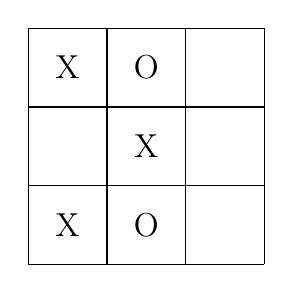
\begin{tikzpicture}
      \foreach \x in {0,1,2,3}
      {\draw (0,\x) -- ++ (3,0);
      \draw (\x,3) -- ++ (0,-3);}
      \node at (0.5,0.5) {\large X};
      \node at (1.5,0.5) {\large O};
      % \node at (2.5,0.5) {\large $3$};
      % \node at (0.5,1.5) {\large $2$};
      \node at (1.5,1.5) {\large X};
      % \node at (2.5,1.5) {\large $2$};
      \node at (0.5,2.5) {\large X};
      \node at (1.5,2.5) {\large O};
      % \node at (2.5,2.5) {\large $3$};
    \end{tikzpicture}
    \capt{Exemple de configuration de jeu au morpion.}
  \end{fig}
\end{exemple}
\examplesol{
\begin{quest}
  \item  $h$ est d’autant plus grande que la position est avantageuse pour $J_1$, et d’autant plus petit que la position est désavantageuse pour $J_2$.
  \item

 \begin{center}
   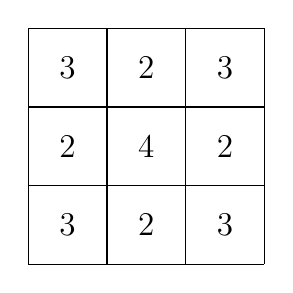
\begin{tikzpicture}
    \foreach \x in {0,1,2,3}
    {\draw (0,\x) -- ++ (3,0);
    \draw (\x,3) -- ++ (0,-3);}
    \node at (0.5,0.5) {\large $3$};
    \node at (1.5,0.5) {\large $2$};
    \node at (2.5,0.5) {\large $3$};
    \node at (0.5,1.5) {\large $2$};
    \node at (1.5,1.5) {\large $4$};
    \node at (2.5,1.5) {\large $2$};
    \node at (0.5,2.5) {\large $3$};
    \node at (1.5,2.5) {\large $2$};
    \node at (2.5,2.5) {\large $3$};
   \end{tikzpicture}
 \end{center}
  % \begin{fig}[]
  %     \centering
  %     
\includegraphics[width=0.3\textwidth]{cases_morpion.png}
  %     % \capt{}
  %   \end{fig}
  \item L’heuristique de cette configuration vaut $h(s) = (3+4+3)-(2+2)=6$. L'heuristique est positive et relativement élevée, ce qui indique que cette configuration de jeu est très avantageuse pour $J_1$ (le joueur qui dessine des croix).
\end{quest}
}
%
% \begin{exemple}{Heuristique pour le puissance 4}
% Prenons l’exemple du Puissance 4 : le but du jeu est d’aligner une suite
% de quatre pions de même couleur sur une grille comptant six rangées et sept colonnes. Tour à tour, les deux
% joueurs placent un pion dans la colonne de leur choix, le pion coulisse alors jusqu’à la position la plus basse
% possible dans la dite colonne à la suite de quoi c’est à l’adversaire de jouer. Le vainqueur est le joueur qui réalise
% le premier un alignement (horizontal, vertical ou diagonal) consécutif d’au moins quatre pions de sa couleur. Si,
% alors que toutes les cases de la grille de jeu sont remplies, aucun des deux joueurs n’a réalisé un tel alignement,
% la partie est déclarée nulle.
%
% \begin{fig}
% \centering
% 
\includegraphics[scale=0.25]{puissance4.png}
% \capt{\footnotesize Dans le jeu Puissance 4, un joueur gagne lorsqu'il réussit à disposer quatre jetons adjacents selon l'horizontale, la verticale, ou la diagonale.}
% \label{fig:puiss4}
% \end{fig}
% %%%%%%%%%%%%%
%
% Une heuristique simple consiste à attribuer à chaque case le nombre d’alignements
% potentiels de quatre pions lorsqu’on place un pion à cet emplacement, puis à sommer les valeurs des cases occupées dans une configuration donnée
% (positivement pour les pions d'Alice, négativement pour ceux de Bob).
% Par exemple, si on convient que les pions jaunes sont ceux d'Alice, la valeur de l’heuristique de configuration $s$
% présentée \Fig{puiss4} est égale à $h(s) =  4 + 5 + 7 + 6 + 8 + 13 + 11 - 3 - 5 - 4 - 8 - 10 - 11 - 11 = 2$.
%
%
% \end{exemple}

%
% %%%%%%%%%%%%%%%%%%%%%
% \begin{figure}[b!]
% \centering
% \subfigure[]{\label{fig:graphe_bi} 
\includegraphics[height=0.35\textwidth]{arene_simple.pdf}}
% \hspace{1cm}
% \subfigure[]{\label{fig:arbre} 
\includegraphics[height=0.35\textwidth]{arbre-crop.pdf}}
% \hspace{1cm}
% \subfigure[]{\label{fig:arbre_h} 
\includegraphics[height=0.35\textwidth]{arbre_h-crop.pdf}}
% %
\includegraphics[scale=0.7]{arene.pdf}
% \caption{\footnotesize (a)~Exemple d'arène d'un jeu d'accessibilité à deux joueurs. Le sommet $0$ (rouge) est le sommet initial. Les sommets $F=\{2,6\}$ (bleus) sont les sommets finaux. Les sommets $S_1=\{0,1,2\}$ (ronds) sont associés au joueur $J_1$, et les sommets $S_2=\{3,4,5\}$ (carrés) au joueur $J_2$. (b) Arbre de décision associé. (c) Heuristique $h(s)$ associé à chaque nœeud de l'arbre.}
% \label{fig:}
% \end{figure}
% %%%%%%%%%%%%%


\parag{Algorithme min-max}
%\parag{Arbre de décision}
 Pour mieux visualiser le caractère séquentiel d’un jeu, on peut lui associer un arbre de décision.
 % Un arbre peut être vu comme un graphe acyclique connexe.
 La \imp{racine} de l’arbre de décision est l’origine, ou sommet initial, du graphe $G=(S,A)$ associé au jeu. Les \imp{nœuds} sont les différents sommets de $S$, en général présents en plusieurs exemplaires ! Les \imp{branches} de l’arbre sont les arcs de $A$ (aussi présents en plusieurs exemplaires en général).  Chaque \imp{feuille} de l’arbre de décision est un sommet final.

 \begin{exemple}{Arbre de décision}
Représenter l’arbre de décision associé au graphe de la \Fig{graphe_bi}.
 \end{exemple}
 \examplesol{
 On voit que dans un arbre de décision, plusieurs nœuds peuvent représenter le même sommet. Il y a donc une certaine redondance. Alors qu'un graphe représente toutes les configurations du jeu, un arbre de décision représente toutes les parties du jeu (chaque parcours possible de l'arbre correspond à une partie). Il y a donc autant de feuilles que de parties possibles.
 \begin{fig}[]
   \centering
   
\includegraphics[scale=0.3]{arbre.png}
   % \capt{}
 \end{fig}
 }
 \medskip

%\parag{Algorithme min-max}
L’algorithme min-max propose une définition récursive simple d’une heuristique à partir des valeurs des feuilles de l’arbre de décision.
% Pour appliquer un algorithme min-max, nous choisirons l’heuristique simple suivante.
% \begin{liste}
% \item $h(s) = +1$ si $s$ est gagnant pour $J_1$.
% \item $h(s) = -1$ si $s$ est perdant pour $J_1$.
% \item $h(s)=0$ si $s$ conduit à une partie nulle (le cas échéant).
% \end{liste}
% Un exemple de calcul d'heuristique est présenté sur l'arbre de la \Fig{arbre_h}.

\begin{theorem}[Algorithme min-max]\label{form:min-max}
\begin{liste}
\item À toute feuille de l’arbre de décision (sommet final) $s \in F$ on attribue
$$
\begin{cases}
   h(s)=+1  & \text{ si } s \in S_1~(J_1 \text{ gagne})  \\
   h(s)=-1 & \text{ si } s \in S_2~(J_1 \text{ perd})
\end{cases}
$$
 % et $h(s)=-1$ si $s \in S_2$ ($J_1$ perd).
%On définit alors $h(s_f)=\pm 1$ pour tout $s_f \in F$ selon ce critère.
\item À tout nœud $s \in J_1$, on attribue à $h(s)$ le \imp{maximum} des heuristiques des sous-arbres.
 % ($J_1$ veut maximiser ses gains).
\item À tout nœud $s \in J_2$, on attribue à $h(s)$ le \imp{minimum} des heuristiques des sous-arbres.
% Si un nœud  $s$ est contrôlé par $J_2$, l’heuristique $h(s)$ vaut le \imp{minimum} des heuristiques de ses sous-arbres ($J_2$ veut minimiser ses pertes).
\end{liste}
\end{theorem}

\begin{exemple}{Algorithme min-max}
Appliquer l’algorithme min-max à l’arbre de décision de l’exemple précédent.
\end{exemple}
\examplesol{

\begin{fig}[]
  \centering
  
\includegraphics[scale=0.4]{arbre_h.png}
  % \capt{}
\end{fig}
}
%En effet, $J_1$ veut maximiser ses gains, et $J_2$ veut minimiser ses pertes.
%
% Sur l'arbre de la \Fig{arbre_h}, on commence par associer les valeurs $\pm 1$ aux feuilles, qui correspondent à des sommets finaux : $+1$ si le sommet final fait gagner Alice, et $-1$ si le sommet final fait gagner Bob. On remonte ensuite l'arbre de proche en proche. Comme il s'agit d'un jeu séquentiel à deux joueurs, chaque niveau de l'arbre correspond à l'un ou l'autre des joueurs. Les sommets $5$ et $6$ appartiennent à Bob : on leur associe le minimum des valeurs des feuilles.  On remonte ensuite aux sommets $1$ et $2$, qui appartiennent à Alice :  on leur associe le minimum des valeurs des nœuds du niveau en-dessous, etc. On voit que le sommet initial $0$ a pour heuristique $h(0) = +1$ : il existe donc une partie gagnante pour Alice.


\begin{prop}\label{prop:}
Un sommet $s \in S_1$ est gagnant pour $J_1$ si et seulement si $h(s)=+1$.
% Il existe alors une stratégie gagnante à partir de $s$.
Il existe une stratégie gagnante pour $J_1$ si et seulement si $h(s_0)=+1$, où $s_0$ est l'origine du graphe. Cette stratégie s’obtient en attribuant à tout nœud $s \in S_1 \backslash F$ un nœud $s_2 \in S_2$ dont l’heuristique vaut $h(s_2)=+1$.
\end{prop}

\begin{exemple}{Algorithme min-max et stratégie gagnante}
  Existe-t-il une stratégie gagnante pour $J_1$ pour l’arbre de décision de l’exemple précédente ? Si oui, déterminer une stratégie gagnante.
\end{exemple}
\examplesol{
Il existe une stratégie gagnante par $h(s_0)=h(0)=+1$. Il en existe plusieurs, mais un exemple est $g : \{0,1\} \rightarrow \{3,4,5,6\}$ telle que $g(0)=4$ et $g(1)=6$, qui permet de parcourir l'arbre en suivant les valeurs d'heuristique $+1$.
}


\subsection{Attracteur}

Soit $F$ l'ensemble des sommets finaux. Parmi ces sommets, certains sont gagnants pour le premier joueur $J_1$. On note $F_1$ cet ensemble. On peut déterminer de proche en proche l'ensemble des sommets gagnants pour $J_1$ (qui permettent d'aboutir à un sommet final de $F_1$) avec la notion d'attracteur.
\begin{exemple}{Notion d'attracteur}
Partons du graphe biparti de la \Fig{graphe_bi}. Les sommets finaux pour $J_1$ sont $F_1 = \{2,3\}$. Nous voyons que le sommet $s=6 \in S_2$ est tel que \emph{tout arc} $(s,s_f)$ partant de $s$ relie un sommet final $s_f$ pour $J_1$. Donc $6$ est une position gagnante pour $J_1$. Effectuons maintenant le même raisonnement sur l'ensemble $A_1(F_1)=\{2,3,6\}$. Il n'existe pas de sommets partant de $S_2$ et aboutissant au sommet $4$, car le graphe est biparti ; mais il existe un sommet $s$ de $S_1$, à savoir le sommet $s=1$,
tel qu’\emph{il existe} un arc $(s,s_g)$ partant de $s$ et aboutissant à une position $s_g \in \{2,3,6\}$ gagnante pour $J_1$. Continuer cette procédure sur l'ensemble $A_2(F_1)=\{2,3,6,1\}$ jusqu'à déterminer la totalité des positions gagnantes.

\begin{fig}[]
  \centering
  
\includegraphics[height=6cm]{A0F1.png}\hspace{1cm}
  
\includegraphics[height=6cm]{A1F1.png}\hspace{1cm}
  
\includegraphics[height=6cm]{A2F1.png}
  % \capt{}
\end{fig}
\end{exemple}
\examplesol{
On trouve $A_3(F_1)=\{2,3,6,1,4,5\}$ puis $A_4(F_1)=\{2,3,6,1,4,5,0\}$, et la procédure s'arrête là puisqu'on a atteint l'origine $0$, qui n'a pas de prédécesseur.
 % On voit en particulier que l'origine $0$ est une position gagnante pour $J_1$, ce qui signifie qu'il existe une stratégie gagnante pour $J_1$ !
}

%Il s'agit du sommet $s=3 \in S_2$. On considère maintenant l'ensemble agrandi $\{6,1,3\}$, etc.

\begin{definition}[Attracteur]
Soit l'ensemble $F_1$ de sommets finaux pour $J_1$ d'une arène $G=(S,A)$.
%L'\imp{attracteur} de $F$ est l'ensemble $A(F)$ obtenu comme limite de la
Soit la suite d'ensemble $\mc{A}_i(F_1)$ définie par récurrence :
\begin{liste}
\item $\mc{A}_0(F_1)=F_1$ ;
\item $\mc{A}_{i+1}(F_1) =  \mc{A}_i(F_1) \cup E_{1\rightarrow i} \cup P_{2 \rightarrow i}$ pour tout $i\geq 0$, où
$$
\begin{cases}
  E_{1 \rightarrow i} & = \{ s_1 \in S_1 \text{ tel que } \exists s_2 \in \mc{A}_i(F_1) \text{ tel que } (s_1,s_2) \in A  \} \\
  P_{2 \rightarrow i} & = \{ s_2 \in S_2 \text{ tel que } \forall (s_2,s_1) \in A, s_1 \in \mc{A}_i(F_1) \}
\end{cases}
$$



\end{liste}
Cette suite est croissante, car $\mc{A}_{i+1}(F_1) \subset \mc{A}_i(F_1)$, et majorée par $S$, donc stationnaire. On note $\mc{A}(F_1)$  et on appelle \imp{attracteur} de $F_1$ l'ensemble limite de la suite $\mc{A}_i(F_1)$.

\end{definition}

\begin{remarque}
  Remarquons qu'à partir de $A_i(F_1)$, le joueur $J_1$ peut atteindre un sommet final en au plus $i$ coups. Si donc $A(F_1) = A_{i}(F_1)$ avec $i$ minimal, $J_1$ peut gagner la partie en $i$ coups (en comptant ceux de $J_2$). Le complémentaire de $A(F_1)$ contient l'ensemble des positions perdantes pour $J_1$, et donc gagnante pour $J_2$. Le calcul d'un attracteur permet ainsi de construire une stratégie gagnante. Ce calcul peut s'effectuer en un temps $\O{n+m}$ où $n$ est le nombre de sommets et $m$ le nombre d'arcs.

\end{remarque}
\begin{prop}\label{prop:}
L'attracteur $\mc{A}(F_1)$ contient l'ensemble des \imp{positions gagnantes} pour $J_1$. Si $\mc{A}(F_1)$ contient l'origine $s_0$, alors il existe une \imp{stratégie gagnante} pour $J_1$.
\end{prop}

\begin{exemple}{Attracteur et stratégie gagnante}
Partons du graphe biparti de la \Fig{graphe_bi}. En combien de coups $J_1$ peut-il gagner la partie ? Proposer une stratégie gagnante et une partie gagnante.
\end{exemple}
\examplesol{
La suite est stationnaire à partir de $\mc{A}_4(F_1)=\{2,3,6,1,4,0\}=\mc{A}(F_1)$, et donc $J_1$ peut gagner la partie en $4$ coups en tout (en comptant ceux de $J_2$). Une stratégie gagnante est $f : \{0,1\} \rightarrow \{4,5,6,7\}$ telle que $f(0) = 4$ et $f(1)=6$.
 % On voit en particulier que l'origine $0$ est une position gagnante pour $J_1$, ce qui signifie qu'il existe une stratégie gagnante pour $J_1$ !
}

\end{document}
